\begin{frame}{Talk outline}
\protect\hypertarget{talk-outline}{}

\begin{itemize}
\tightlist
\item
  What is streaming data?
\item
  Computational models for streaming data
\item
  Statistical models for streaming data
\item
  An example: nowcasting urban rainfall events
\end{itemize}
\bigskip

Joint work with: Andy Golightly, Naomi Hannaford, Sarah Heaps, Yuanzhi Huang, Stephen Johnson, Kevin Wilson, \ldots

\bigskip

Funding from UKRI-NERC and The Alan Turing Institute

\end{frame}

\begin{frame}{Streaming data applications}
\protect\hypertarget{streaming-data-applications}{}

\begin{itemize}
\tightlist
\item
  Streaming voice and video applications

  \begin{itemize}
  \tightlist
  \item
    Zoom, Netflix, YouTube, Spotify, etc.
  \item
    Typically streamed directly \emph{over the internet} to your display
  \item
    Even if the video is downloaded to local storage, it is still
    \emph{streamed} from storage and decompressed on-the-fly for
    real-time viewing - the entire video is never fully decompressed in
    RAM - not just about moving data over the internet
  \end{itemize}
\item
  Real-time financial market trading data

  \begin{itemize}
  \tightlist
  \item
    Automated trading systems
  \item
    Decision support for human traders
  \end{itemize}
\item
  On-line processing (and compression) of scientific experiments

  \begin{itemize}
  \tightlist
  \item
    Biological sequencing technologies, neuroscience data
  \item
    Collider experiments, astronomical surveys
  \end{itemize}
\item
  Real time sensor network data for continuous monitoring

  \begin{itemize}
  \tightlist
  \item
    Traffic (and pollution) monitoring, weather forecasting, healthcare
    wearables, \ldots{}
  \end{itemize}
\end{itemize}

\end{frame}

\begin{comment}

\begin{frame}{Turing Fellow project}
\protect\hypertarget{turing-fellow-project}{}

\begin{block}{Streaming data modelling for real-time monitoring and
forecasting}

\begin{itemize}
\item
  Computational architecture and infrastructure
\item
  Statistical methodology and algorithms
\item
  Case studies: Urban Analytics (The Urban Observatory - eg. air
  pollution), Healthcare (neuroscience), engineering biology, \ldots{}
\end{itemize}

\emph{Joint work with A Golightly, S Heaps, Y Huang, N Hannaford, A
Hardy, \ldots{}}

\end{block}

\end{frame}


\end{comment}


\begin{frame}{Streaming data architecture}
\protect\hypertarget{streaming-data-architecture}{}

\begin{block}{Fundamental concepts}

\begin{itemize}
\tightlist
\item
  A \emph{stream} is a (possibly infinite) sequence of values of a given
  (potentially complex) data type, with a definite order
\item
  The stream is accessed one value at a time, and processing is done
  incrementally, triggered by the arrival of each value
\item
  Typically only \emph{one pass} over the data is possible
\item
  Streams are connected together in a DAG called the \emph{flow graph}
\end{itemize}

\end{block}

\begin{block}{Software libraries and frameworks}

\begin{itemize}
\tightlist
\item
  \emph{Storm}, \emph{Heron}, \emph{Spark streaming}, \emph{Akka
  streams}, \emph{Flink}, \emph{Kafka streams} are well-known examples
  of streaming data frameworks
\item
  Frameworks are often run on the \emph{JVM}, built in languages with
  good support for \textbf{functional programming} (FP), such as
  \emph{Scala}, and rely to a greater-or-lesser extent on FP principles
  such as \emph{functional reactive programming} (FRP)
\end{itemize}

\end{block}

\end{frame}

\begin{frame}[fragile]{Functional models of streaming data}
\protect\hypertarget{functional-models-of-streaming-data}{}

\begin{itemize}
\tightlist
\item
  A key streaming data processing abstraction is a pure
  \textbf{function}:
  \[h: \mathcal{X} \times \mathcal{Y} \longrightarrow \mathcal{X}\]
\end{itemize}

\begin{Shaded}
\begin{Highlighting}[]
\NormalTok{advance: (State, Observation) => State}
\end{Highlighting}
\end{Shaded}

combining current world knowledge (encapsulated in a \texttt{State})
together with the latest observation to get an updated world view

\begin{itemize}
\tightlist
\item
  Then given
  \(x_0\in\mathcal{X},\quad \mathbf{y} \in \mathcal{Y}^{\mathbb{N}}\)
\end{itemize}

\begin{Shaded}
\begin{Highlighting}[]
\NormalTok{s0: State, sObs: Stream[Observation]}
\end{Highlighting}
\end{Shaded}

we transform the stream of observations \(\mathbf{y}\) to states
\(\mathbf{x}\in\mathcal{X}^{\mathbb{N}}\):

\begin{Shaded}
\begin{Highlighting}[]
\NormalTok{sState: Stream[State] = sObs.}\FunctionTok{scan}\NormalTok{(s0)(advance)}
\end{Highlighting}
\end{Shaded}

via successive application of \(h\).

\end{frame}

\begin{frame}[fragile]{Stream transformation}
\protect\hypertarget{stream-transformation}{}

Streams are \emph{functors}, since they \texttt{map}:

\begin{Shaded}
\begin{Highlighting}[]
\NormalTok{  Stream[A].}\FunctionTok{map}\NormalTok{[B](f: A => B): Stream[B]}
\end{Highlighting}
\end{Shaded}

The \texttt{scan} operation, sometimes called \texttt{scanLeft}, has
signature:

\begin{Shaded}
\begin{Highlighting}[]
\NormalTok{  scanLeft[B](init: B)(advance: (B, A) => B): Stream[B]}
\end{Highlighting}
\end{Shaded}

For example:

\begin{Shaded}
\begin{Highlighting}[]
\KeywordTok{val}\NormalTok{ naturals = Stream.}\FunctionTok{iterate}\NormalTok{(}\DecValTok{1}\NormalTok{)(_ + }\DecValTok{1}\NormalTok{)}
\CommentTok{// 1, 2, 3, 4, ...}
\KeywordTok{val}\NormalTok{ evens = naturals }\FunctionTok{map}\NormalTok{ (_ * }\DecValTok{2}\NormalTok{)}
\CommentTok{// 2, 4, 6, 8, ...}
\KeywordTok{val}\NormalTok{ triangular = naturals.}\FunctionTok{scan}\NormalTok{(}\DecValTok{0}\NormalTok{)(_ + _).}\FunctionTok{drop}\NormalTok{(}\DecValTok{1}\NormalTok{)}
\CommentTok{// 1, 3, 6, 10, ...}
\end{Highlighting}
\end{Shaded}

\end{frame}

\begin{frame}[fragile]{State-space modelling}
\protect\hypertarget{state-space-modelling}{}

In state-space modelling, we have a

\begin{itemize}
\tightlist
\item
  forward model: \(X_t | x_{t-1} \sim f(x_t|x_{t-1})\) or
  \texttt{f:\ X\ =\textgreater{}\ P{[}X{]}}
\item
  and observation model: \(Y_t|x_t \sim g(y_t|x_t)\) or
  \texttt{g:\ X\ =\textgreater{}\ P{[}Y{]}}
\end{itemize}

where \texttt{P{[}\_{]}} is a suitable \emph{probability monad}, and
\(f\), \(g\) are \emph{Markov kernels}.

For \emph{filtering} we typically think in terms of predict-update
steps:

\begin{itemize}
\tightlist
\item
  \(p(x_{t-1}|\mathcal{Y}_{t-1}) \rightarrow p(x_t|\mathcal{Y}_{t-1})\)
  or \texttt{predict:\ P{[}X{]}\ =\textgreater{}\ P{[}X{]}}
\item
  \(p(x_t|\mathcal{Y}_{t-1}) \rightarrow p(x_t|\mathcal{Y}_t)\) or
  \texttt{update:\ (P{[}X{]},Y)\ =\textgreater{}\ P{[}X{]}}
\end{itemize}

\texttt{predict} is monadic \texttt{flatMap} (or
\texttt{\textgreater{}\textgreater{}=}) with \texttt{f}, and
\texttt{update} is \emph{probabilistic conditioning} (Bayesian updating)
via \texttt{g}

Streaming:
\texttt{advance\ =\ update\ compose\ predict\textquotesingle{}} where
\texttt{State\ =\ P{[}X{]}} - eg. one step of a Kalman or particle
filter

\end{frame}

\begin{frame}{Composable functional models of on-line algorithms and
PPLs}
\protect\hypertarget{composable-functional-models-of-on-line-algorithms-and-ppls}{}

\begin{itemize}
\item
  Once we start to think about filtering in terms of operations
  involving probability monads and Markov kernels, it becomes easier to
  think about how to make models and algorithms composable and scalable,
  and about the connection to \emph{probabilistic programming} and
  monadic \emph{probabilistic programming languages} (PPLs)
\item
  Possible to think about all of the standard models and algorithms for
  SSMs within this framework: Kalman filters (regular, extended,
  unscented, ensemble, \ldots{}), particle filters (bootstrap, SIR,
  auxiliary, \ldots{}), etc.
\end{itemize}

\textbf{Law, W (2019)} Functional probabilistic programming for scalable
Bayesian modelling, \emph{arXiv}, 1908.02062

\end{frame}

\begin{comment}

\begin{frame}{POMP models}
\protect\hypertarget{pomp-models}{}

\begin{itemize}
\tightlist
\item
  Classical SSMs assume that the data are on a regular equispaced time
  grid, so that the state evolution model \(f(x_t|x_{t-1},\theta)\)
  represents a single time step of the process
\item
  Many sensors and devices do not generate data on a regular grid,
  either by design, or due to crashes/reboots creating large gaps of
  missing values, pushing observations onto a \emph{misaligned grid}, or
  changes in sampling frequency, etc.
\item
  \textbf{Partially observed Markov process} (POMP) models generalise
  classical SSMs in two important ways:

  \begin{itemize}
  \tightlist
  \item
    The state evolution model formulated in \emph{continuous time}, and
    is described by a transition kernel \(f(x_{t+t'}|x_t,t',\theta)\)
  \item
    It is not (necessarily) required that the transition kernel can be
    \emph{evaluated} --- only that the state process can be
    stochastically \emph{simulated} forwards in time
  \end{itemize}
\end{itemize}

\end{frame}

\begin{frame}{On-line filtering of POMP models}
\protect\hypertarget{on-line-filtering-of-pomp-models}{}

\begin{itemize}
\tightlist
\item
  The ``bootstrap'' particle filter is a ``likelihood free'' algorithm
  for sequentially computing the filtering distribution of a POMP model
  (for fixed \(\theta\)): \[
  \pi(x_t|\mathcal{Y}_t),\ \text{ where } \mathcal{Y}_t \equiv \{y_s|y_s\in\mathcal{Y},s\leq t\}
  \]
\item
  Although it is typically presented in discrete time, it works fine for
  continuous time processes observed discretely at irregular times
\item
  Additionally, composable (and tractable) families of continuous time
  transition kernels can be built using similar techniques as are
  sometimes used for discrete time DLMs
\end{itemize}

\textbf{Law \& W (2018)}
\href{https://doi.org/10.1007/s11222-017-9783-1}{Composable models for
online Bayesian analysis of streaming data}, \emph{Statistics and
Computing}, \textbf{28}:1119-37.

\end{frame}

\end{comment}

\begin{frame}{What makes an algorithm ``on-line''?}
\protect\hypertarget{what-makes-an-algorithm-on-line}{}

\begin{itemize}
\tightlist
\item
  Not all streaming data applications are about time series
\item
  Many are just about analysing data based on a single pass
\item
  Almost any statistical algorithm can be expressed in the form of a
  streaming data algorithm
\item
  All of the data observed so far can be embedded in the \emph{state},
  and any analysis whatsoever of the data can be restarted from scratch
  with the arrival of each new observation!
\item
  We wouldn't consider such an analysis to be \emph{genuinely} on-line
\item
  We typically assume that the ``size'' of the state is bounded, and
  that the computational ``complexity'' of the \emph{advance} step has
  bounded expectation
\end{itemize}

\end{frame}

\begin{frame}{Spatio-temporal modelling}
\protect\hypertarget{spatio-temporal-modelling}{}

\begin{block}{Spatio-temporal SSMs}

\begin{itemize}
\tightlist
\item
  SSMs/POMPs fit naturally into the streaming data framework
\item
  Can be ``on-line'', since the \textbf{Markov property} for the hidden
  state process facilitates the bounding of state size and computation
  associated with updating
\end{itemize}

\end{block}

\begin{block}{Spatio-temporal GPs}

\begin{itemize}
\tightlist
\item
  Relatively straightforward to formulate GPs sequentially and embed in
  a streaming data framework
\item
  Most commonly used space-time covariance functions don't lead to
  simple Markov properties, so special techniques for ``scalable'' and
  ``streaming'' GPs must be used to ensure the algorithms are genuinely
  ``on-line''
\end{itemize}

\end{block}

\end{frame}

\begin{comment}

\begin{frame}{Scalable GP modelling}
\protect\hypertarget{scalable-gp-modelling}{}

\begin{itemize}
\tightlist
\item
  As the number of observations, \(n\), grows, the \(n\times n\)
  covariance (or precision) matrix gradually becomes problematic
  (whether inversion is explicit or not)
\item
  Can subset or merge design points in more-or-less principled ways, or
  form some other sparse or low-rank approximation of the covariance (or
  precision) matrix
\item
  There is also interest in learning GP hyper-parameters (such as length
  scales) in an on-line fashion
\item
  Hybrid approaches using off-line algorithms for learning static
  (hyper)parameters and on-line algorithms for dynamic state work well
  in practice
\item
  Very active research area
\end{itemize}

\end{frame}

\begin{frame}[fragile]{Example application: pollution monitoring}
\protect\hypertarget{example-application-pollution-monitoring}{}

\begin{block}{The Urban Observatory: \texttt{urbanobservatory.ac.uk}}

\begin{itemize}
\tightlist
\item
  The largest set of publicly available real time urban data in the UK
  --- web API (and also a \emph{websocket} for real time data)
\item
  eg. Temperature, rainfall and air quality sensors around the city
\item
  Rainfall radar data
\item
  \emph{Multivariate}, \emph{spatial}, \emph{temporal},
  \emph{irregularly observed}, \emph{mixed modality} (eg. point and
  areal)
\end{itemize}

\end{block}

\begin{block}{Pollution mapping in real time}

\begin{itemize}
\tightlist
\item
  Pollution monitors at various (fixed) locations around the city
\item
  Measurements every few minutes from every sensor, but not on a fixed
  grid, and not temporally aligned across sensors
\item
  Would like to ``nowcast'' a spatially continuous map of pollution
  levels across the city, updated with each new observation
\end{itemize}

\end{block}

\end{frame}

\begin{frame}{Pollution monitoring application}
\protect\hypertarget{pollution-monitoring-application}{}

\begin{itemize}
\tightlist
\item
  Urban observatory provides APIs (and a websocket) for accessing
  multiple air pollution measurements (eg. CO, NO2, NO, O3, PM1, PM4,
  PM10, PM25)
\item
  New small stream processing application server (in Scala), consuming a
  live stream of pollution measurements from an array of sensors around
  the city, updating a spatio-temporal GP in real-time, generating a new
  stream containing a now-casting pollution map (with uncertainty), for
  consumption by a small web front-end visualisation application (in JS)
\item
  Front-end application consumes nowcast map stream (via a websocket)
  and renders in a web page
\end{itemize}

\end{frame}

\begin{frame}{Pollution nowcasting}
\protect\hypertarget{pollution-nowcasting}{}

\begin{figure}
\centering
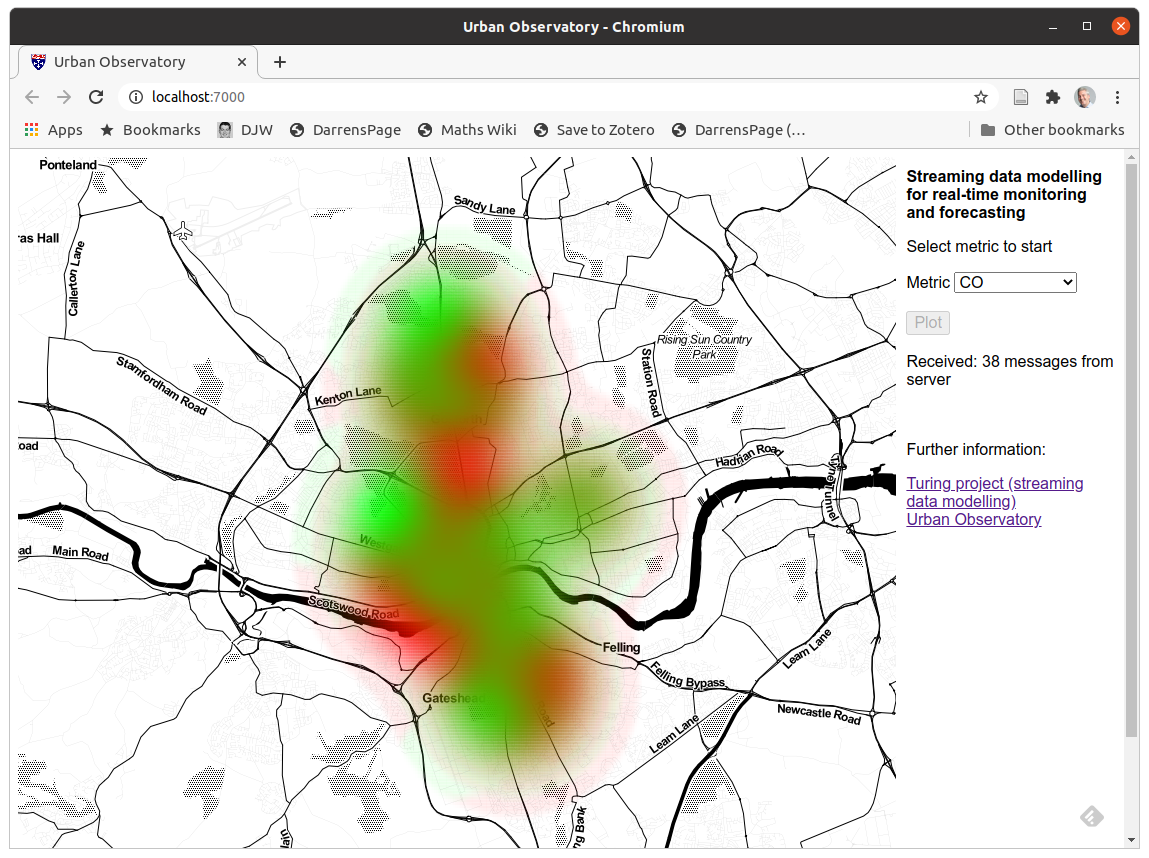
\includegraphics{uo-gui.png}
\caption{UO ``live'' monitoring}
\end{figure}

\end{frame}

\begin{frame}{Practical issues}
\protect\hypertarget{practical-issues}{}

\begin{itemize}
\tightlist
\item
  We have a running test-bed system that can visualise pollution levels
  across the city, using transparent fade-out to represent uncertainty
  in areas of poor sensor coverage, updating in real-time as each new
  observation arrives
\item
  Many practical issues requiring further work and collaboration with
  subject matter experts before public deployment
\item
  Modelling issues

  \begin{itemize}
  \tightlist
  \item
    Modelling sensor-specific issues and biases --- impact of biases on
    parameter inference --- especially length scales
  \item
    Incorporation of expert prior information
  \item
    Independent calibration and verification of maps, especially against
    areal data
  \end{itemize}
\item
  Visualisation issues

  \begin{itemize}
  \tightlist
  \item
    Colour-scales for inferred pollution levels
  \item
    Appropriate, calibrated visualisation of uncertainty
  \end{itemize}
\end{itemize}

\end{frame}

\begin{frame}{Current and future plans and projects}
\protect\hypertarget{current-and-future-plans-and-projects}{}

\begin{itemize}
\tightlist
\item
  Complete work on the air pollution case study
\item
  Neuroscience application
\item
  Engineering biology application
\item
  Complete rainfall modelling work
\item
  Collaboration on novel streaming data architectures
\item
  Further work on scalable sequential Bayesian updating methodology
\item
  Software for (functional) probabilistic programming on streaming data
\end{itemize}

\end{frame}

\end{comment}


\begin{frame}{Flood-PREPARED (NERC-funded)}
\protect\hypertarget{flood-prepared-nerc-funded}{}

\begin{block}{Predicting Rainfall Events by Physical Analytics of
REaltime Data}

\begin{itemize}
\tightlist
\item
  Real-time short-term high-resolution spatio-temporal rainfall
  modelling, synthesising \emph{areal} weather radar and \emph{point}
  rain gauge data
\item
  Near real-time emulation of and data assimilation for a hydrodynamic
  urban flood model
\item
  Hooked up to traffic monitors, CCTV feeds, social media sources, etc.,
  all live streaming (from the Urban Observatory), for the development
  of an emergency decision support system for Newcastle
\end{itemize}

\textbf{Johnson, Heaps, Wilson, W (2021)} Bayesian spatio-temporal model
for high-resolution short-term forecasting of precipitation fields,
\emph{arXiv}, 2105.03269

\end{block}

\end{frame}

\begin{frame}[fragile]
\frametitle{Motivation}
\bigskip
\bigskip
\begin{itemize}
\item \alert{Flood PREPARED} --- \emph{Predicting Rainfall Events by Physical Analytics of REaltime Data}
  \item Large NERC (UK) funded multi-disciplinary project at Newcastle, involving engineers, hydrological modellers, computer scientists, statisticians, ... 
\item Make cities more resilient to surface water flooding
\item Real-time analysis to allow for earlier and more geographically precise warning
\item Use-case focusing on Newcastle-upon-Tyne, UK
  \item Data feeds from Newcastle's Urban Observatory project:  \alert{\url{http://urbanobservatory.ac.uk/}}
\end{itemize}
\end{frame}


\begin{frame}[fragile]
\frametitle{Our challenges}
\bigskip
\begin{itemize}
\item  Develop a probabilistic spatio-temporal rainfall model
\medskip
\begin{itemize}
\item make use of all available rain-related data sources
\medskip
\item be able to forecast rainfall intensity in real-time
\medskip
\item high-resolution in both space and time
\end{itemize} 
\bigskip
\item Predictions from our model will form inputs for a hydrological flood model
\medskip
\begin{itemize}
\item Hydrological flood model takes input on a regular lattice grid
\end{itemize}
\bigskip
\item There is a second phase concerned with \emph{data assimilation} for the hydrological urban flood model, but not discussing that today
\end{itemize}
\end{frame}


\begin{frame}{Synthesising point and areal data (Flood-PREPARED)}
\protect\hypertarget{synthesising-point-and-areal-data-flood-prepared}{}

\begin{figure}
\centering
\includegraphics{ncl_z2_radar_grid_gauge.pdf}
\caption{Rainfall data}
\end{figure}

\end{frame}


\begin{frame}
\frametitle{Rain field evolution}
\begin{itemize}
\item Suppose the (latent) rain field process exists on a regular lattice grid containing $N$ locations
\bigskip
\item $\theta_{t,i,j} \in \mathbb{R}$ denotes location $(i,j)$ at time $t$
\begin{itemize}
\medskip
\item $\theta_{t,i,j} > 0 \Longrightarrow$ rainfall mm/h
\medskip
\item $\theta_{t,i,j} \leq 0 \Longrightarrow$ zero rainfall 
\end{itemize}
\bigskip
\item Suppose location $(i,j)$ is influenced by its first order neighbours from previous time step
\medskip
\[
\begin{matrix}
    & \theta_{t,i-1,j} & \\
    \theta_{t,i,j-1} & \theta_{t,i,j} & \theta_{t,i,j+1} & \\
    & \theta_{t,i+1,j} &  \\
\end{matrix} \to \quad \theta_{t+1,i,j}
\]
\end{itemize}
\end{frame}


\begin{frame}
\begin{itemize}
\item Specifically
\begin{align*}
\theta_{t+1,i,j} = \beta_1 \theta_{t,i,j} + \beta_2 \theta_{t,i,j-1} + &\beta_3 \theta_{t,i-1,j} \\
& + \beta_4 \theta_{t,i+1,j} + \beta_5  \theta_{t,i,j+1} + \; \textit{noise}
\end{align*}
\item Let $\thetavec_t =  ( \theta_{t,1:\nr,1}, \theta_{t,1:\nr,2},\dots,\theta_{t,1:\nr,\nc})^\text{T}$
\bigskip
\item Evolution is
\begin{equation*}
\thetavec_t = G \thetavec_{t-1} + \vec{w}_t, \qquad \vec{w}_t \sim \N_N(\vec{0}, W_t),
\end{equation*}
\begin{equation*}
``G" =  \begin{bmatrix}
. & \beta_3 & .\\
\beta_2 & \beta_1 & \beta_5\\
. & \beta_4 & .\\
\end{bmatrix}
\end{equation*}
\end{itemize}
\end{frame}

\begin{comment}

\frame{
\frametitle{STAR(1) (forward) model}
\begin{center}
\movie{\includegraphics[height=0.85\textheight]{star1frame}}{../19-05-Montreal/fig/star1prior.mp4}
\end{center}
}

\end{comment}


\begin{frame}
\frametitle{Gauge data}
\begin{itemize}
\item Each of the $\Ng$ rain gauges are within a single grid cell
\begin{itemize}
\medskip
\item numerous gauges may be within the same grid cell
\end{itemize}
\medskip
\item Let $\tilde{y}^\g_{ti}$ be observation from gauge $i$ at time $t$
\begin{itemize}
\medskip
\item observations are in mm/h
\end{itemize}
\medskip
\item The measurements of the latent rain field ($\tilde{y}^\g_{ti}$) are censored below zero
\medskip
\item Treat observations of zero as \textit{unobserved} (negative) values
\medskip
\item Suppose there exists a (partially observed) process $\vec{Y}_t^\g \in \mathbb{R}^\Ng$ such that
\begin{equation*}
\qquad \qquad \tilde{Y}_{ti}^\g = Y_{ti}^\g \; \mathbb{I}(Y_{ti}^\g > 0), \qquad \text{for} \; i=1,\dots,\Ng.
\end{equation*}
\end{itemize}
\end{frame}

\begin{frame}
\begin{itemize}
\bigskip
\item Assume
\begin{equation*}
\qquad  \Ygt = \mathcal{I}^\g \thetavec_t + \mu^\g \vec1 +  \gamG + \vec\epsilon^\g_t,  \qquad \vec\epsilon^{\g}_t \sim \N_\Ng(\vec0,(1/\phig) \INGNG ),
\end{equation*}
\bigskip
\vspace{-0.7cm}
\item  $\mathcal{I}^\g$ is an $\Ng \times N$ dimensional matrix where row~$i$ contains a 1 in the column corresponding to the grid location of rain gauge~$i$, and zeros in the remaining columns
\bigskip
\item $\mu^\g \in \mathbb{R}$ represents the mean gauge observation
\bigskip
\item $\gamG \in \mathbb{R}^\Ng$ is a vector of gauge specific biases (random effects)
\bigskip
\item $\phig \in \mathbb{R}_{>0}$ is the gauge precision
\end{itemize}
\end{frame}



\begin{frame}
\frametitle{Radar data}
\begin{itemize}
\item Radar provides radar reflectivity factor, Z
\bigskip
\item The Z/R relation is
\[
Z = aR^b
\]
where $R$ is the rain rate in mm/h
\bigskip
\item $a$ and $b$ depend on the rain droplet distribution
\bigskip
\item Typically $a \in (200,600)$ and $b \in(1.4,2.0)$
\begin{itemize}
\medskip
\item we choose $a=296$ and $b = 1.47$
\end{itemize}
\end{itemize}
\end{frame}


\begin{comment}
\begin{frame}
\begin{itemize}
\bigskip
\item Radar observations are not equally distributed over the field
\medskip
\begin{itemize}
\item elevation angle of $3^\circ$ 
\medskip
\item radial resolution of $150$m
\medskip
\item angular resolution of $1^\circ$
\end{itemize}
\bigskip
\item Map (converted) radar observations $R$ onto the lattice grid
\bigskip
\item Let $\tilde{y}^\tr_{ti}$ be the average of the values that fall within grid cell $i$
\bigskip
\item The measurements of the latent rain field ($\tilde{y}^\tr_{ti}$) are censored below zero
\bigskip
\end{itemize}
\end{frame}
\end{comment}

\begin{frame}
\begin{itemize}
\item Treat observations of zero as \textit{unobserved} (negative) values
\bigskip
\item Suppose there exists a (partially observed) process $\vec{Y}_t^\tr \in \mathbb{R}^N$ such that
\begin{equation*}
\qquad \qquad \tilde{Y}_{ti}^\tr = Y_{ti}^\tr  \; \mathbb{I}(Y_{ti}^\tr > 0), \qquad \text{for} \; i=1,\dots,N.
\end{equation*}
\item Assume
\begin{equation*}
\qquad  \qquad  \vec{Y}_t^\tr = \psi \thetavec_t + \mu^\tr \vec1 + \vec\epsilon^{\text{r}}_t,    \qquad \vec\epsilon^{\text{r}}_t \sim \N_N(\vec0,1/\phir \INN )
\end{equation*}
\item $\psi \in \mathbb{R}$ is a scaling parameter to calibrate the radar observations to the rain field
\medskip
\item $\mu^\tr \in \mathbb{R}$ represents the mean radar field
\medskip
\item $\phir \in \mathbb{R}_{>0}$ is the radar precision
\end{itemize}
\end{frame}


\begin{frame}
\frametitle{The model}
The full model is
\begin{align*}
\hspace{2cm} \tilde{\vec{Y}}_{t}^\tr &= \vec{Y}_{t}^\tr  \; \mathbb{I}(\vec{Y}_{t}^\tr > \vec{0}), \\
 \tilde{\vec{Y}}_{t}^\g &= \vec{Y}_{t}^\g  \; \mathbb{I}(\vec{Y}_{t}^\g > \vec{0}), \\
\Yrt &= \psi \thetavec_t + \mu^\tr \vec1 + \vec\epsilon^{\text{r}}_t,   & \vec\epsilon^{\text{r}}_t &\sim \N_N(\vec0,1/\phir \INN ), \\
\Ygt &= \mathcal{I}^\g \thetavec_t + \mu^\g \vec1 + \gamG + \vec\epsilon^\g_t,  &\vec\epsilon^{\g}_t &\sim \N_\Ng(\vec0,1/\phig \INGNG ), \\
\thetavec_t &= G\thetavec_{t-1} + \vec{w}_t, & \vec{w}_t &\sim \N_{N}(\vec0,1/\phi^\theta \INN),
\end{align*}
\bigskip
where
\begin{equation*}
``G" =  \begin{bmatrix}
. & \beta_3 & .\\
\beta_2 & \beta_1 & \beta_5\\
. & \beta_4 & .\\
\end{bmatrix}
\end{equation*}
\end{frame}

\begin{frame}
  \frametitle{Model semantics}
  \begin{itemize}
\item  The radar data provides a useful high-resolution overview of where rain is, and where it is moving
\item Rain gauge data is useful for calibrating the radar data in terms of actual water hitting the ground
  \end{itemize}
\end{frame}




\begin{frame}
\frametitle{Censored DLM}
If we let $\tilde{\vec{y}}_t=
\left(\begin{matrix}
\tilde{\vec{y}}_t^\tr \\
\tilde{\vec{y}}_t^\g
\end{matrix}\right)$, then an equivalent model specification is
\begin{align*}
\hspace{1cm} \tilde{\vec{Y}}_{t} &= \vec{Y}_{t}^*  \; \mathbb{I}(\vec{Y}_{t}^* > \vec{0}), \\
\Yt  &= \vec{Y}_{t}^* - (\mu^\tr \lrvec + \mu^\g \lgvec + \Mg\gamG) \\
\Yt  &= F \thetavec_t  + \vec{v}_t, & \vec{v}_t &\sim \N_{N+\Ng}(\vec0,V ),\\
\thetavec_t &= G\thetavec_{t-1} + \vec{w}_t, & \vec{w}_t &\sim \N_{N}(\vec0,1/\phi^\theta \INN),
\end{align*}
\bigskip
where
\[
F = 
\begin{bmatrix}
\psi \INN \\
\mathcal{I}^\g
\end{bmatrix},
\qquad
V = 
\begin{bmatrix}
1/\phir \INN & 0_{N\times\Ng}\\
0_{\Ng\times N} & 1/\phig \INGNG
\end{bmatrix}
\]
\end{frame}




\subsection{Bayesian Inference}
\begin{frame}
\frametitle{Bayesian Inference via MCMC}
\bigskip
\begin{itemize}
\item Let $\D_o=\{\tilde{y}^\tr_{ti},\tilde{y}^\g_{tj} : \tilde{y}_{ti}^\tr \neq 0 \lor \tilde{y}_{tj}^\g \neq 0, \forall \; t,i,j \}$ be the collection of \textit{observed data}
\bigskip
\item Let $\D_c=\{\tilde{y}^\tr_{ti},\tilde{y}^\g_{tj} : \tilde{y}_{ti}^\tr = 0 \lor \tilde{y}_{tj}^\g=0, \forall \; t,i,j \}$ be the collection of censored (\textit{unobserved}) data
\bigskip
\item Let $\vec{\rho}= ( \phir,\phig,\betavec,\mu^\tr,\mu^\g,\psi,\gamG)$
\bigskip
\item Unknown parameters are $(\thetavec_{0:T}$, $\vec{\rho}, \D_c)$

\end{itemize}
\end{frame}


\begin{frame}
\frametitle{Bayesian Inference via MCMC}
\bigskip
\begin{itemize}
\item Given a ``sensible'' prior it is fairly straightforward to draw posterior samples of $\vec{\rho}$ from $\pi(\vec\rho|\D_o,\D_c,\thetavec_{0:T})$
\bigskip
\item It is also straightforward to draw from $\pi(\D_c|\D_o,\vec\rho,\thetavec_{0:T})$
\bigskip
\item State inference is typically achieved by drawing $\thetavec_{0:T}$ from $\pi(\thetavec_{0:T}|\D, \vec\rho)$ using the FFBS algorithm
\bigskip
\item Unfortunately the FFBS algorithm is not practical when the dimension of the state and/or observation is large
\end{itemize}
\end{frame}



\begin{comment}
\begin{frame}
\frametitle{FFBS Issues}
\begin{itemize}
\item Each component of $(\thetavec_{0:T}, \vec{Y}_{1:T})$ is Gaussian $\Longrightarrow$ all marginal/conditional distributions are also Gaussian
\bigskip
\item The Kalman Filter is a mechanism for determining the first and second moments of all the relevant Gaussian distributions
\bigskip
\item We can then ``backwards sample'' from the appropriate distributions to obtain (Gibbs) draws for $\thetavec_{0:T}$
\bigskip
\item A general FFBS algorithm is
\medskip
\begin{itemize}
\item Run the Kalman Filter
\medskip
\item For $t=T,\dots,0$ draw $\thetavec_t| \cdot \sim \N_N(\cdot,\cdot)$
\end{itemize}
\end{itemize}
\end{frame}


\begin{frame}
\frametitle{The Kalman Filter}
\small
Assuming $\thetavec_0 \sim \N_N(\mvec_0,C_0)$, then for each time $t=1,\dots$
\begin{itemize}
\item The one-step-ahead predictive distribution of the states is
\[
\thetavec_t|\vec{y}_{1:t-1} \sim \N_N(\vec{a}_t,R_t) \qquad \text{where} \qquad 
\begin{matrix*}[l]
\vec{a}_t = G_t \mvec_{t-1} \\
R_t = G_tC_{t-1}G_t' + W_t\\
\end{matrix*} 
\]
\item The one-step-ahead predictive distribution of the observations is
\[
\vec{Y}_t|\vec{y}_{1:t-1} \sim \N_N(\vec{f}_t, Q_t) \qquad \text{where} \qquad 
\begin{matrix*}[l]
\vec{f}_t = F_t \vec{a}_t \\
 Q_t = F_tR_tF_t' + V_t
\end{matrix*} \hspace{0.5cm}
\] 
\item The filtering distribution of the state at time $t$ is
\[
\phantom{_{-1}} \thetavec_t|\vec{y}_{1:t} \sim \N_N(\mvec_t,C_t) \qquad \text{where} \qquad
\begin{matrix*}[l]
\mvec_t = \vec{a}_t + K_t\vec{e}_t \\
C_t = R_t - K_tF_tR_t
\end{matrix*} \
\] 
$\vec{e}_t = \vec{y}_t-\vec{f}_t$ is the residual error and $K_t = R_tF_t'Q_t^{-1}$ is the Kalman gain
\end{itemize}
\end{frame}


\begin{frame}
\frametitle{The Kalman Filter}
\small
Assuming $\thetavec_0 \sim \N_N(\mvec_0,C_0)$, then for each time $t=1,\dots$
\begin{itemize}
\item The one-step-ahead predictive distribution of the states is
\[
\thetavec_t|\vec{y}_{1:t-1} \sim \N_N(\vec{a}_t,R_t) \qquad \text{where} \qquad 
\begin{matrix*}[l]
\vec{a}_t = G_t \mvec_{t-1} \\
\red{R_t = G_tC_{t-1}G_t' + W_t}\\
\end{matrix*} 
\]
\item The one-step-ahead predictive distribution of the observations is
\[
\vec{Y}_t|\vec{y}_{1:t-1} \sim \N_N(\vec{f}_t, Q_t) \qquad \text{where} \qquad 
\begin{matrix*}[l]
\vec{f}_t = F_t \vec{a}_t \\
\red{ Q_t = F_tR_tF_t' + V_t}
\end{matrix*} \hspace{0.5cm}
\] 
\item The filtering distribution of the state at time $t$ is
\[
\phantom{_{-1}} \thetavec_t|\vec{y}_{1:t} \sim \N_N(\mvec_t,C_t) \qquad \text{where} \qquad
\begin{matrix*}[l]
\mvec_t = \vec{a}_t + K_t\vec{e}_t \\
\red{C_t = R_t - K_tF_tR_t}
\end{matrix*} \
\] 
$\vec{e}_t = \vec{y}_t-\vec{f}_t$ is the residual error and \red{$K_t = R_tF_t'Q_t^{-1}$} is the Kalman gain
\end{itemize}
\end{frame}

\end{comment}


\begin{frame}
\frametitle{The Ensemble Kalman Smoother (EnKS)}
\bigskip
\begin{itemize}
\item The EnKS is an approximate (forward only) method for obtaining posterior draws from $\pi(\thetavec_{0:T}|\D, \vec\rho)$
\bigskip
\item Consider a collection of~$\Ne$ particles (an ensemble) that are ``draws'' from the appropriate distributions
\bigskip
\item Propagate and shift the particles such that the expectation and variance (of the ensemble members) is that of the true distribution
\bigskip
\item Exact samples of $\thetavec_{0:T}$ are obtained as $\Ne \to \infty$ 
\end{itemize}
\end{frame}


\begin{frame}
\small
Initialise: draw $\vec\theta_{0|0}^j \indep \N_N(\mvec_0, C_0)$ for $j=1,\dots,\Ne$ \\
For $t=1,\dots,T$
\begin{enumerate}
\item Forecast step: for $j=1,\dots,\Ne$
\begin{itemize}
\item Let $\tilde\thetavec_\tgtm^j = G\thetavec_\tmgtm^j$ 
\item Let $\thetavec_\tgtm^j = \tilde\thetavec_\tgtm^j + \vec{w}_t^j$ where  $\vec{w}^j_t \indep \N_N(\vec{0},W_t)$ 
\end{itemize}
\item Smoothing step: for $j=1,\dots,\Ne$
\begin{itemize}
\item Generate pseudo-observations $\tilde{\vec{y}}^j_t = F_t \vec{\theta}_\tgtm^j + \vec{v}_t^j$ where $\vec{v}_t^j \indep \N_N(\vec{0}, V_t)$
\item For $\ell=0,\dots,t$
\begin{itemize}
\item Compute (the smoothed state) $\vec\theta_{\ell|t}^j = \vec\theta_{\ell|t-1}^j + \hat{K}_{\ell,t}(\vec{y}_t - \tilde{\vec{y}}^j_t)$
\end{itemize}
\end{itemize}
\end{enumerate}
$\hat{K}_{\ell,t} = \Sigma_{\ell,\tgtm}^{\theta y} \left( \Sigma_{t,\tgtm}^{yy} \right)^{-1}$ is the (ensemble based) approx Kalman gain \\
\phantom{row} 
$\Sigma^{\theta y}_{\ell t|t-1} = \text{Cov}(\Theta_{\ell|t-1},\tilde{Y}_\tgtm)$ is the sample cross-covariance of the ensembles of states $\Theta_{\ell|t-1}$ and pseudo observations $\tilde{Y}_\tgtm$
\end{frame}



\begin{frame}
  \frametitle{Real data analysis}
  \mbox{} \hfill $N = 36 \times 36$ \quad $\Ne=100$
\begin{figure}[h!]
\begin{center}
        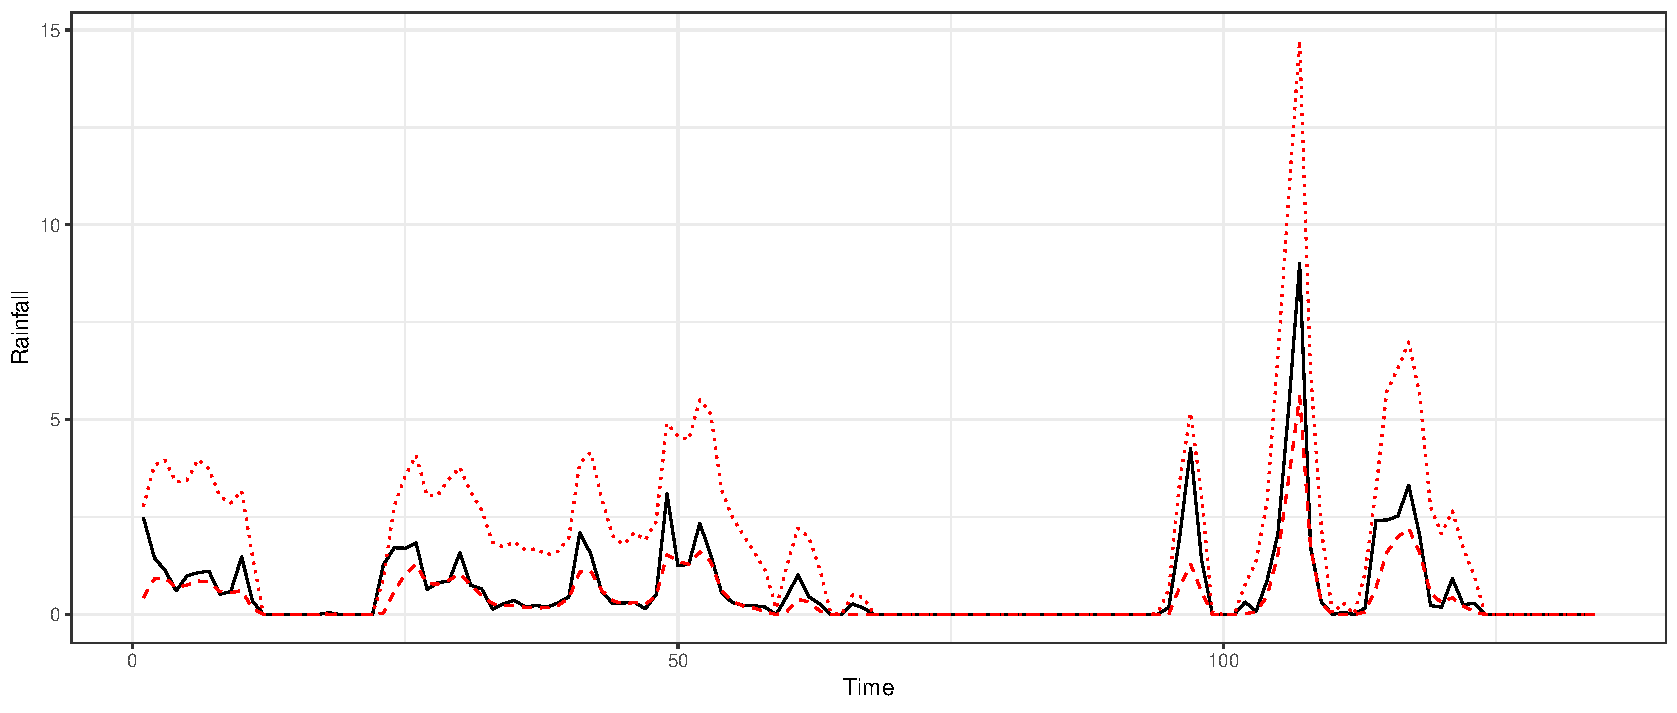
\includegraphics[width=0.8\linewidth, clip, trim = 0 0 0 0]{post_med_uq_radar_location.pdf} \vspace{0.5cm}
                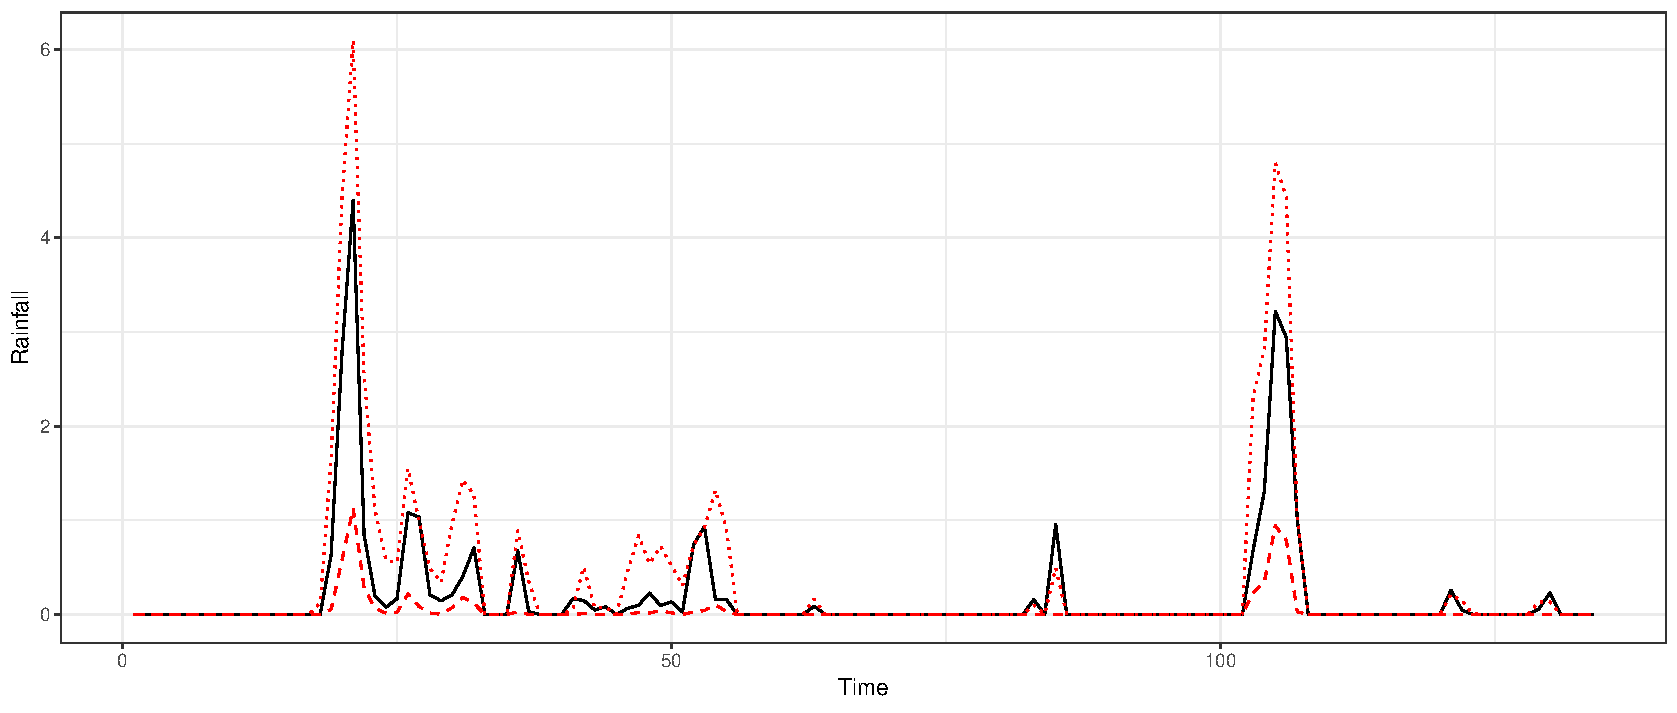
\includegraphics[width=0.8\linewidth, clip, trim = 0 0 0 0]{post_med_uq_radar_location_2.pdf}
\end{center}
\end{figure}
\end{frame}

\begin{frame}
  \frametitle{Deployment in the live demonstrator system}
  \begin{itemize}
  \item The model is deployed into the live demonstrator in two components
  \item Static parameter estimation is run off-line, but regularly updated
  \item Conditional on the static parameters, the short-term forecasting model is run on-line, generating forecasted spatio-temporal rainfall fields
  \item The forecasted rainfall fields are used as input for the hydrodynamical urban flood-forecasting model
    \item The urban flood forecasting model is run on-line and coupled to other decision support components
  \end{itemize}
\end{frame}

\begin{frame}
\centerline{\includegraphics[height=\textheight]{h_3600}}
\end{frame}

\begin{frame}
\centerline{\includegraphics[height=\textheight]{h_7200}}
\end{frame}

\begin{frame}
\centerline{\includegraphics[height=\textheight]{h_10800}}
\end{frame}

\begin{frame}
  \frametitle{Application Summary}
  \begin{itemize}
  \item Censored continuous fields can be a useful model for spatial data containing many zeros
  \item Lattice Markov spatio-temporal models can be cast in the DLM framework
    \item Serious computational challenges associated with large spatio-temporal models
%  \item Complex models, data, inference and forecasting algorithms lead to non-trivial software engineering challenges in addition to the usual algorithmic and computational challenges
%  \item CS principles of modularity and compositionality are important for developing scalable and re-usable models and algorithms
%    \item Statisticians have many powerful (exact) Monte Carlo Bayesian inference algorithms appropriate for both state and parameter inference for Markov processes, but these don't always scale well to very high dimensions
  \item EnKF algorithms can be usefully embedded into Bayesian parameter inference algorithms
    \item EnKF/S can be useful for sampling (tractable) DLMs (in preference to FFBS) if the state dimension is very high
  \end{itemize}
  \vfill

% \alert{\url{darrenjw.github.io}} \hfill \url{@darrenjw}
  
\end{frame}



\begin{frame}{Summary}
\protect\hypertarget{summary}{}

\begin{itemize}
\tightlist
\item
  The analysis and modelling of streaming data is becoming increasingly
  important
\item
  Typical motivations:

  \begin{enumerate}
  \tightlist
  \item
    Sequential analysis of ``live'' data in (near) real time
  \item
    Analysis of large data-sets based on ``one pass'' methods
  \item
    Parallel computation via stream \emph{splitting} and \emph{merging}
  \end{enumerate}
\item
  There exist computational models and software libraries for working
  with streaming data in an efficient and robust way
\item
  Functional (and reactive) programming languages and approaches are
  well-suited to working with (infinite) data streams (and probabilistic
  programs)
\item
  Time series are a natural fit to streaming data models, but not all
  streaming data applications have a natural temporal aspect
\item
  Many statistical models and algorithms can be adapted to a sequential
  context \hfill \alert{\url{darrenjw.github.io}}
\end{itemize}

\end{frame}
